% !TEX root = main.tex
\begin{subsection}{A Partial Upper Bound}\label{sec:IntroMainThm}
In this section, we show how to compute an upper bound on $\rho$, with a user-defined confidence $\beta \in (0, 1)$. We do this by constructing a $l$-step CQLF which is valid with probability at least $\beta$. Note that, the existence of a $l$-step CQLF implies $\rho \leq 1$ due to Theorem \ref{thm:cqlf}.

Let us analyze the relationship between the solutions of the theoretical optimization problem \eqref{eqn:campiOpt2} and the practical version \eqref{eq:lowerbound}, with finitely many constraints. Even though in practice, one would solve the optimization problem  \eqref{eq:lowerbound} as suggested in the previous section, for the sake of rigor and clarity of our proofs, we introduce a slighly different optimization problem. In this new optimization problem, an objective function is considered, and a ``regularization parameter'', $\eta > 0$, is added. As the reader will see, we will derive results valid for arbitrarily small values of $\eta$, and so this will not hamper the practical accuracy of our technique, while allowing us to derive a theoretical asymptotic guarantee (i.e. for large number of observations).

\begin{equation}\label{eqn:campiOpt03}
\begin{aligned}
& \text{min}_{P} & & \lambda_{\max}(P) \\
& \text{s.t.} 
&  & (A_{j_l} A_{j_{l-1}} \dots A_{j_1} x)^T P (A_{j_l} A_{j_{l-1}} \dots A_{j_1} x) \leq {((1 +\eta)\gamma^*(\omega_N))}^{2l} x^T P x,\\
&&&\qquad \qquad \qquad \qquad \qquad \qquad \qquad \qquad \quad \qquad \forall (x, j_{1},\dots, j_{l}) \in \omega_N \subset Z_l \\
& && P \succeq I, \\
\end{aligned}
\end{equation}
where $Z_l:= \sphere \times M^l$, $\eta > 0$, and $\gamma^*(\omega_N)$ is the optimal solution to the optimization problem \eqref{eq:lowerbound}. Recall that $\omega_N$ is a given uniform random sample on the set $Z_l$ and of size $N$. 

For the rest of the discussion, we refer to the optimization problem \eqref{eqn:campiOpt03} by $ \Opt(\omega_N)$. We denote its optimal solution by $P(\omega_N)$. We drop the explicit dependence of $P$ on $\omega_N$ when it is clear from the context. There are a few points that are worth noting about \eqref{eqn:campiOpt03}. Firstly, due to Property \ref{property:homogeneity}, we can replace the constraint $P \succ 0$ with the constraint $P \succeq I$. Moreover, for reasons that will become clear later in the discussion, we chose the objective function as $\lambda_{\max}(P)$, instead of solving a feasibility problem in $P$. Lastly, the additional $\eta$ factor is introduced to ensure strict feasibility of \eqref{eqn:campiOpt03}, which will be helpful in the following discussion.

The curious question whether the optimal solution of the sampled problem $\Opt(\omega_N)$ is a feasible solution to \eqref{eqn:campiOpt1} has been widely studied in the literature \cite{campi}. It turns out that under certain technical assumptions, one can bound the proportion of the constraints of the original problem \eqref{eqn:campiOpt1} that are violated by the optimal solution of \eqref{eqn:campiOpt03}, with some probability which is a function of the sample size $N$. 

In the following theorem, we adapt a classical result from random convex optimization literature to our problem.



\begin{thm}[adapted from Theorem 3.3\footnotemark, \cite{campi}]\label{mainTheorem0}
Let $d$ be the dimension of $\Opt(\omega_N)$ and $N \geq d+1$. Consider the optimization problem $\Opt(\omega_N)$ given in \eqref{eqn:campiOpt03}, where $\omega_N$ is a uniform random sample drawn from the set $Z_l$.
Then, for all $\varepsilon \in (0,1]$ the following holds:
\begin{equation}\label{eqn:violation}
\mu_l^N\hspace{-1mm}\left\{ \omega_N \in Z_l^N: \mu_l(V(\omega_N)) \leq \varepsilon \right\}\hspace{-1mm} \geq 1- \sum_{j=0}^{d} \binom{N}{j}\varepsilon^j (1-\varepsilon)^{N-j},
\end{equation}
where $\mu_l^N$ denotes the product probability measure on $Z_l^N$, and $V(\omega_N)$ is defined by \small{
\begin{equation*} 
\begin{aligned}
& V(\omega_N) := \{z=(x,j_{1},\dots,j_{l}) \in Z_l: \\
& (A_{j_l} A_{j_{l-1}} \dots A_{j_1} x)^T P(\omega_N)(A_{j_l} A_{j_{l-1}} \dots A_{j_1} x) > (\gamma_{\omega_N}^{*})^{2l} x^T P(\omega_N) x\},
\end{aligned}
\end{equation*}
}
i.e., it is the set of constraints that are violated by the optimal solution of $\Opt(\omega_N)$. From now we will denote the left hand-side of \eqref{eqn:violation} by $\beta$.
\end{thm}

\footnotetext{Theorem 3.3 in \cite{campi} requires $\Opt(\omega_N)$ to satisfy the following technical assumptions:\begin{enumerate}
\item When the problem $\Opt(\omega_N)$ admits an optimal solution, this solution is unique.
\item Problem $\Opt(\omega_N)$ is nondegenerate with probability $1$.
\end{enumerate}
Here, the first assumption can be enforced if required by adding a tie-breaking rule to $\Opt(\omega_N)$ as explained in Appendix A in \cite{tiebreak}, while the second assumption can be lifted, as explained in PART 2b in \cite{nondegen}, thanks to the introduction of a ``constraint heating''.
}


\begin{cor}\label{cor:gettingRidOfm}
Consider a set of matrices $\mathcal{M}$, $\gamma^{*}$ optimal solution of \eqref{eq:lowerbound} and matrix $P \succ 0$ optimal solution of $\Opt(\omega_N)$. Then $P$ will satisfy:
\begin{equation}\label{eqn:P0}
\begin{aligned}
& (A_{j_l} A_{j_{l-1}} \dots A_{j_1} x)^T P(A_{j_l} A_{j_{l-1}} \dots A_{j_1} x) \leq (\gamma^{*})^{2l} x^T P x, \\
& \qquad \qquad \qquad \qquad \forall\, x \in \sphere \setminus \sphere', \forall\ (j_1, \dots, j_l) \in M^l,
\end{aligned}
\end{equation}
for some $\sphere' \subset \sphere$ such that $\sigma^{n-1}(\sphere') \leq \varepsilon m^l $.
\end{cor}

The proof of Corollary~\ref{cor:gettingRidOfm} is based on straightforward arguments on measures, and is given in Appendix~\ref{proof:cor_m}. This result allows us to only consider set of violating points on the sphere from now. Note that, this result is conservative: the case where we have the equality $\sigma(\sphere') = \varepsilon m^l$ corresponds to the case where we have only observed one mode, and have then minimal knowledge on the system for a given $\varepsilon$.


The above results allow us to conclude, from a finite number of observations, that with probability $\beta$ (where $\beta$ goes to $1$ as $N$ goes to infinity), the required property is actually satisfied for the complete sphere $\sphere$, except on a small set of measure at most $\varepsilon m^l$. This means that, the ellipsoid computed by $\Opt(\omega_N)$ is ``almost invariant"  except on a set of measure bounded by $\varepsilon m^l$. This can be representend in the case $n=2$ by the following plot, where the points of the ellipse in red are points that might violate the contractivity constraint (the set of red points has measure at most $\varepsilon m^l$).

\begin{figure}[H]\label{fig:ellipsoid}
\begin{center}
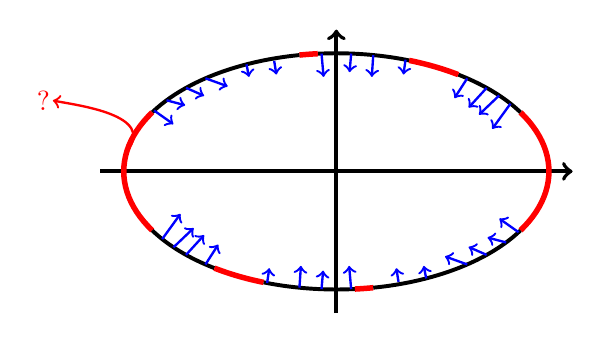
\begin{tikzpicture}[scale=0.6]
%\draw (-0.1,-0.1) -- (0.1,0.1);
%\draw (-0.1,0.1) -- (0.1,-0.1);

\draw[line width=0.5mm,black,->] (-5,0) -- (5,0);
\draw[line width=0.5mm,black,->] (0,-3) -- (0,3);

\draw [line width = 0.7mm,red,domain=-30:30] plot ({4.5 * cos(\x)}, {2.5 * sin(\x)});
\draw [line width = 0.5mm,black,domain=30:55] plot ({4.5 * cos(\x)}, {2.5 * sin(\x)});
\draw [line width = 0.7mm,red,domain=55:70] plot ({4.5 * cos(\x)}, {2.5 * sin(\x)});
\draw [line width = 0.5mm,black,domain=70:95] plot ({4.5 * cos(\x)}, {2.5 * sin(\x)});
\draw [line width = 0.7mm,red,domain=95:100] plot ({4.5 * cos(\x)}, {2.5 * sin(\x)});
\draw [line width = 0.5mm,black,domain=100:150] plot ({4.5 * cos(\x)}, {2.5 * sin(\x)});
\draw [line width = 0.7mm,red,domain=150:210] plot ({4.5 * cos(\x)}, {2.5 * sin(\x)});
\draw [line width = 0.5mm,black,domain=210:235] plot ({4.5 * cos(\x)}, {2.5 * sin(\x)});
\draw [line width = 0.7mm,red,domain=235:250] plot ({4.5 * cos(\x)}, {2.5 * sin(\x)});
\draw [line width = 0.5mm,black,domain=250:275] plot ({4.5 * cos(\x)}, {2.5 * sin(\x)});
\draw [line width = 0.7mm,red,domain=275:280] plot ({4.5 * cos(\x)}, {2.5 * sin(\x)});
\draw [line width = 0.5mm,black,domain=280:330] plot ({4.5 * cos(\x)}, {2.5 * sin(\x)});

\draw[->,line width=0.3mm,red] (-4.432,0.434) .. controls (-3.8,1.2) and (-5.5,1.4) .. (-6,1.5);
\draw[red] (-6.2,1.5) node {?};

\draw[->,line width = 0.3mm,blue] (3.6862,1.4339) -- (3.3,0.9);
\draw[->,line width = 0.3mm,blue] (3.4472,1.6070) -- (3.02,1.2);
\draw[->,line width = 0.3mm,blue] (3.182,1.7678) -- (2.8,1.35);
\draw[->,line width = 0.3mm,blue] (2.7705,1.97) -- (2.5,1.55);
\draw[->,line width = 0.3mm,blue] (-3.6862,-1.4339) -- (-3.3,-0.9);
\draw[->,line width = 0.3mm,blue] (-3.4472,-1.6070) -- (-3.02,-1.2);
\draw[->,line width = 0.3mm,blue] (-3.182,-1.7678) -- (-2.8,-1.35);
\draw[->,line width = 0.3mm,blue] (-2.7705,-1.97) -- (-2.5,-1.55);
\draw[->,line width = 0.3mm,blue] (1.4651,2.3638) -- (1.42,2.05);
\draw[->,line width = 0.3mm,blue] (0.7814,2.4620) -- (0.75,2);
\draw[->,line width = 0.3mm,blue] (0.3139,2.4939) -- (0.28,2.1);
\draw[->,line width = 0.3mm,blue] (-0.3139,2.4939) -- (-0.27,2);      
\draw[->,line width = 0.3mm,blue] (-1.4651,-2.3638) -- (-1.42,-2.05);
\draw[->,line width = 0.3mm,blue] (-0.7814,-2.4620) -- (-0.75,-2);
\draw[->,line width = 0.3mm,blue] (-0.3139,-2.4939) -- (-0.28,-2.1);
\draw[->,line width = 0.3mm,blue] (0.3139,-2.4939) -- (0.27,-2);
\draw[->,line width = 0.3mm,blue] (-1.3157,2.33908) -- (-1.27,2.05);
\draw[->,line width = 0.3mm,blue] (-1.9018,2.2658) -- (-1.85,2);
\draw[->,line width = 0.3mm,blue] (-2.7705,1.97) -- (-2.3,1.8);
\draw[->,line width = 0.3mm,blue] (-3.182,1.7678) -- (-2.8,1.6);      
\draw[->,line width = 0.3mm,blue] (-3.5939,1.5045) -- (-3.2,1.4); 
\draw[->,line width = 0.3mm,blue] (-3.8573,1.2876) -- (-3.45,1); 
\draw[->,line width = 0.3mm,blue] (1.3157,-2.33908) -- (1.27,-2.05);
\draw[->,line width = 0.3mm,blue] (1.9018,-2.2658) -- (1.85,-2);
\draw[->,line width = 0.3mm,blue] (2.7705,-1.97) -- (2.3,-1.8);
\draw[->,line width = 0.3mm,blue] (3.182,-1.7678) -- (2.8,-1.6);      
\draw[->,line width = 0.3mm,blue] (3.5939,-1.5045) -- (3.2,-1.4); 
\draw[->,line width = 0.3mm,blue] (3.8573,-1.2876) -- (3.45,-1); 
\end{tikzpicture}
\end{center}
\caption{Representation of the ``partial invariance property'' obtained by application of the results in \ref{mainTheorem0}. A priori, we know nothing about the images of the red points. Our goal is to convert this partial invariance property into a global stability property.}
\end{figure}
Thus, we are left with the following question: ``What can we conclude on the JSR if we can assume that the Lyapunov property is satisfied by all points, except a set of measure $\varepsilon m^l$?''
\end{subsection}


\begin{subsection}{The Spherical Case}\label{sec:pbsphere}
We consider first the special and simpler case when the ellipse defined by $P$ is in fact a sphere, and more specifically the unit sphere $\sphere$. The set of points that can violate the constraint still has measure bounded by $\varepsilon m^l$, and is now denoted by $X_{\varepsilon m^l}$. We will see that for this precise case our question becomes a geometric problem, which we describe and solve in this section. Our reasoning uses the following fundamental property of switched linear systems.

\begin{property}\label{property:convpres}
The dynamics given in \eqref{eq:switchedSystem} is convexity-preserving, meaning that for any set of points $X \subset \mathbb{R}^n$ we have:
$$ f(\conv({X}))\subset \conv(f(X)). $$
\end{property}

This leads us to look for the largest sphere in $\convhull (S \setminus X_{\varepsilon m^l})$. By homogeneity of the system, this sphere will be centered at the origin, and we denote by $\delta$ its radius. We consider this sphere $\sphere_{\delta}$ since, by Property~\ref{property:convpres}, we know that the $l$-traces by system~\eqref{eq:switchedSystem} initialized in $\sphere_{\delta}$ (hence initialized in $\convhull (S \setminus X_{\varepsilon m^l})$), will lie in $\convhull (f(S \setminus X_{\varepsilon m^l})) \subset \gamma^{l} \ball$. Then, the rate of growth of $\sphere_{\delta}$ after $l$ steps will be upper bounded by $\frac{(\gamma^{*})^{l}}{\delta}$.

\begin{figure}[H]
\begin{center}
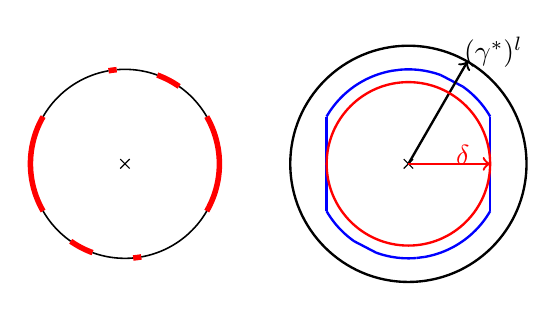
\begin{tikzpicture}[scale=0.6]
\draw (0.1,-0.1) -- (-0.1,0.1);
\draw (0.1,0.1) -- (-0.1,-0.1);
\draw[line width = 0.7mm,red,domain=-30:30] plot ({2*cos(\x)}, {2*sin(\x)});
\draw[line width = 0.2mm,black,domain=30:55] plot ({2 * cos(\x)}, {2 * sin(\x)});
\draw[line width = 0.7mm,red,domain=55:70] plot ({2 * cos(\x)}, {2 * sin(\x)});
\draw[line width = 0.2mm,black,domain=70:95] plot ({2 * cos(\x)}, {2 * sin(\x)});
\draw[line width = 0.7mm,red,domain=95:100] plot ({2 * cos(\x)}, {2 * sin(\x)});
\draw[line width = 0.2mm,black,domain=100:150] plot ({2 * cos(\x)}, {2 * sin(\x)});
\draw[line width = 0.7mm,red,domain=150:210] plot ({2 * cos(\x)}, {2 * sin(\x)});
\draw[line width = 0.2mm,black,domain=210:235] plot ({2 * cos(\x)}, {2 * sin(\x)});
\draw[line width = 0.7mm,red,domain=235:250] plot ({2 * cos(\x)}, {2 * sin(\x)});
\draw[line width = 0.2mm,black,domain=250:275] plot ({2 * cos(\x)}, {2 * sin(\x)});
\draw[line width = 0.7mm,red,domain=275:280] plot ({2 * cos(\x)}, {2 * sin(\x)});
\draw[line width = 0.2mm,black,domain=280:330] plot ({2 * cos(\x)}, {2 * sin(\x)});

\draw (6.1,-0.1) -- (5.9,0.1);
\draw (6.1,0.1) -- (5.9,-0.1);
\draw[line width = 0.3mm,blue,domain=30:55] plot ({6 + 2 * cos(\x)}, {2 * sin(\x)});
\draw[line width = 0.3mm,blue,domain=70:95] plot ({6 + 2 * cos(\x)}, {2 * sin(\x)});
\draw[line width = 0.3mm,blue,domain=100:150] plot ({6 + 2 * cos(\x)}, {2 * sin(\x)});
\draw[line width = 0.3mm,blue,domain=210:235] plot ({6 + 2 * cos(\x)}, {2 * sin(\x)});
\draw[line width = 0.3mm,blue,domain=250:275] plot ({6 + 2 * cos(\x)}, {2 * sin(\x)});
\draw[line width = 0.3mm,blue,domain=280:330] plot ({6 + 2 * cos(\x)}, {2 * sin(\x)});

\draw[line width=0.3mm,blue] ({6 + 2*cos(-30)}, {2*sin(-30)}) -- ({6 + 2*cos(30)}, {2*sin(30)});
\draw[line width=0.3mm,blue] ({6 + 2*cos(55)}, {2*sin(55)}) -- ({6 + 2*cos(70)}, {2*sin(70)});
\draw[line width=0.3mm,blue] ({6 + 2*cos(95)}, {2*sin(95)}) -- ({6 + 2*cos(100)}, {2*sin(100)});
\draw[line width=0.3mm,blue] ({6 + 2*cos(150)}, {2*sin(150)}) -- ({6 + 2*cos(210)}, {2*sin(210)});
\draw[line width=0.3mm,blue] ({6 + 2*cos(235)}, {2*sin(235)}) -- ({6 + 2*cos(250)}, {2*sin(250)});
\draw[line width=0.3mm,blue] ({6 + 2*cos(275)}, {2*sin(275)}) -- ({6 + 2*cos(280)}, {2*sin(280)});

\draw[line width=0.3mm,black] (6,0) circle[radius=2.5cm];
\draw[line width=0.3mm,black,->] (6,0) -- (7.25,{2.5*sin(60)});
\draw[line width=0.3mm,black] (7.8,{2.5*sin(60)+0.2}) node {$(\gamma^{*})^l$};
\draw[line width=0.3mm,red] (6,0) circle[radius=1.73cm];
\draw[line width=0.3mm,red,->] (6,0) -- (7.73,0);
\draw[line width=0.3mm,red] (7.15,0.2) node {$\delta$};
\end{tikzpicture}
\caption{On the left, our problem in the case of a sphere. On the right, we represent in blue the boundary of the convex hull of the points satisfying the $(\gamma^{*})^l$-contractivity constraint on $l$-traces; in red we represent the largest sphere $\sphere_{\delta}$ included in that convex hull ; in black we represent the boundary of the set where elements of all $l$-traces initialized in that convex hull can lie.}
\end{center}
\end{figure}

We investigate then the case for which the largest ball included $\convhull (S \setminus X_{\varepsilon m^l})$ has the smallest radius $\delta$. This will maximize our upper bound on the growth of rate of the sphere $\sphere_{\delta}$ considered, and thus will give us an upper bound on the JSR equal to $\frac{\gamma^{*}}{\sqrt[l]{\delta}}$. Minimizing $\delta$ will then give us the worst case set for a given measure $\varepsilon m^l$ of points authorized to violate our constraint. This worst case will happen when the set of violating points on $\sphere$ is a spherical cap (see Proposition~\ref{thm:mainSphericalCap} below). Let us define this notion.

\begin{defn}
We define the \emph{spherical cap} on $\sphere$ for a given hyperplane $c^Tx = k$ as:
\begin{equation*}
\mathcal{C}_{c,k} := \{x \in \sphere : c^Tx >k\}.
\end{equation*}
\end{defn}

\begin{figure}[H]
\begin{center}
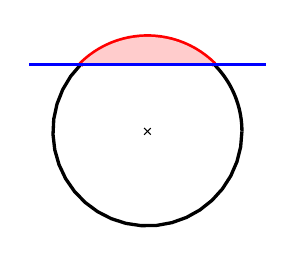
\begin{tikzpicture}[scale=0.6]
\draw (-0.07,-0.07) -- (0.07,0.07);
\draw (-0.07,0.07) -- (0.07,-0.07);
\draw [black,very thick,domain=0:45] plot ({2*cos(\x)}, {2*sin(\x)});
\draw [line width = 0.7mm,red,domain=45:135] plot ({2*cos(\x)}, {2*sin(\x)});
\draw [black,very thick,domain=135:360] plot ({2*cos(\x)}, {2*sin(\x)});
\fill[fill=red!20] (1.414,1.414) arc [start angle=45, end angle=135, radius=2] -- cycle;
\draw[blue, very thick] (-2.5,1.414) -- (2.5,1.414);
\end{tikzpicture}
\end{center}
\caption{A spherical cap in the case $n=2$. The hyperplane $c^Tx =k$ defining the spherical cap is in blue, the spherical cap is in red.}
\end{figure}

We now define the function 
\begin{equation}\label{shrinkage}
\Delta: \left\{
    \begin{split}
    &\wp(\sphere) \to [0,1]\\ 
    &X \mapsto \sup \{r: r\ball \subset \conv(\sphere \setminus X)\}.
    \end{split}
  \right.
\end{equation}

Note that, $\Delta(X)$ can be rewritten as:
\begin{equation}\label{shrinkage2}
\Delta(X) =  \dist(\partial  \conv(\sphere \setminus X), 0).
\end{equation}

The following proposition tells us that $\Delta$ is minized when $X$ is a spherical cap, i.e., the radius $\delta$ of our largest sphere $\sphere_{\delta}$ will be reached when $X_{\varepsilon m^l}$ is a spherical cap.

\begin{prop}\label{thm:mainSphericalCap}
Let $\mathcal{X}_{\varepsilon m^l} = \{X \subset \sphere: \sigma^{n-1}(X) \leq \varepsilon m^l\}$. Then, for any $\varepsilon \in (0,1/m^l]$, the function $\Delta(X)$ attains its minimum over $\mathcal{X}_{\varepsilon m^l}$ for some $X$ which is a spherical cap.
\end{prop}

We give a proof of Proposition~\ref{thm:mainSphericalCap} in Appendix~\ref{sec:app_prelim_caps}.

By Property \ref{property:homogeneity} (homogeneity of the system), we have $x \in V_{\sphere} \iff -x \in V_{\sphere}$,  which implies that $X_{\varepsilon m^l}$ will be in fact union of two spherical caps, each of measure $\frac{\varepsilon m^l}{2}$. We denote from now $\varepsilon':=\frac{\varepsilon m^l}{2}$. We illustrate the problem when $X_{\varepsilon m^l}$ is of this form.

\begin{figure}[H]
\begin{center}
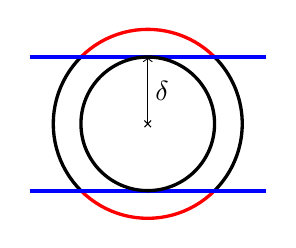
\begin{tikzpicture}[scale=0.6]
\draw (-0.07,-0.07) -- (0.07,0.07);
\draw (-0.07,0.07) -- (0.07,-0.07);
\draw [black,very thick,domain=0:45] plot ({2*cos(\x)}, {2*sin(\x)});
\draw [red,very thick,domain=45:135] plot ({2*cos(\x)}, {2*sin(\x)});
\draw [black,very thick,domain=135:225] plot ({2*cos(\x)}, {2*sin(\x)});
\draw [red,very thick,domain=225:315] plot ({2*cos(\x)}, {2*sin(\x)});
\draw [black,very thick,domain=315:360] plot ({2*cos(\x)}, {2*sin(\x)});
\draw[line width = 0.5mm,blue] (-2.5,1.414) -- (2.5,1.414);
\draw[line width = 0.5mm,blue] (-2.5,-1.414) -- (2.5,-1.414);
\draw[->] (0,0) -- (0,1.414);
\draw (0.3,0.7) node {$\delta$};
\draw [black,very thick] (0,0) circle [radius = 1.414cm];
\end{tikzpicture}
\end{center}
\caption{Illustration of the situation giving the minimal $\delta$, for $n=2$. The set $V(\omega_N)$ is represented in red, and is the union of two spherical caps, each of measure $\varepsilon'$.}
\end{figure}


For a given spherical cap of area measure $\varepsilon'$, we can compute a closed form expression of the radius of the corresponding largest ball. We denote by $\alpha$ the function that associates to each $\varepsilon' \in (0,1/2]$ the value of this radius. We have an expression for $\alpha$ given by the following lemma (see the Appendix~\ref{sec:ProofSphericalCaps} for details of its proof).

\begin{lem}\label{lemma:propositionSphericalCaps}
Let $\varepsilon \in (0, \frac{1}{2}]$ and $\alpha: [0,1] \to \mathbb{R}_{\geq 0}$ be defined by:
\begin{equation}\label{eqn:ballinc}
\alpha(\varepsilon) := \inf_{X \in \mathcal{X}_{\varepsilon}} \sup\{r: r\ball \subset \convhull(\sphere \setminus X)\},
\end{equation}
where $\mathcal{X}_{\varepsilon} = \{ X \subset \sphere: \sigma^{n-1}(X) \leq \varepsilon \}$. Then, $\alpha(\varepsilon)$ is given by the formula:
\begin{equation}\label{eqn:alphaEpsilon}
\alpha(\varepsilon) = \sqrt{1- I^{-1} \left( 2\varepsilon; \frac{n-1}{2}, \frac{1}{2} \right)}, 
\end{equation}
where $I$ is the regularized incomplete beta function.
\end{lem}

By exploiting Property \ref{property:convpres} and Lemma~\ref{lemma:propositionSphericalCaps} above, we can now show in Lemma \ref{lemma:epsilon1} how one can compute an upper bound on the JSR when the ``almost invariant" set is the unit sphere $\sphere$.

\begin{prop}\label{lemma:epsilon1}
Let $\varepsilon \in (0, 1/m^l)$ and $\gamma^{*} \in \mathbb{R}_{> 0}$. Consider the set of matrices $\mathcal{M}$ and $A \in \mathcal{M}^l$ satisfying:
\begin{equation}\label{eqn:contraction}
\begin{aligned}
& (A_{j_l} A_{j_{l-1}} \dots A_{j_1} x)^T (A_{j_l} A_{j_{l-1}} \dots A_{j_1} x) \leq (\gamma^{*})^{2l} x^Tx, \\
& \forall\, x \in \sphere \setminus \sphere', \forall\,(j_1, \dots, j_l) \in M^l,
\end{aligned}
\end{equation}
where $\sphere' \subset \sphere$ and $\sigma^{n-1}(\sphere') \leq \varepsilon m^l$, then we have:
\begin{equation*}
\rho(\mathcal{M}) \leq \frac{\gamma^{*}}{\sqrt[l]{\alpha(\frac{\varepsilon m^l}{2})}}
\end{equation*}
where $\alpha(\frac{\varepsilon m^l}{2})$ is given in \eqref{eqn:alphaEpsilon}.
\end{prop}


\begin{pf}
Note that, \eqref{eqn:contraction} implies that:
$(A_{j_l} A_{j_{l-1}} \dots A_{j_1}) (\sphere \setminus \sphere') \subset \gamma^l \ball.$
Using Property \ref{property:convpres} this also implies:
$$A_{j_l} A_{j_{l-1}} \dots A_{j_1} \left( \convhull(\sphere \setminus \sphere') \right) \subset \convhull \left( A_{j_l} A_{j_{l-1}} \dots A_{j_1}(\sphere \setminus \sphere') \right) \subset \gamma^l \ball .$$
Then, by Lemma~\ref{lemma:propositionSphericalCaps}, we have:
$$A_{j_l} A_{j_{l-1}} \dots A_{j_1} \left( \alpha(\varepsilon) \ball \right) \subset A_{j_l} A_{j_{l-1}} \dots A_{j_1} \left( \convhull (\sphere \setminus \sphere') \right) \subset \gamma^l\ball, \quad  \forall\, (j_1, \dots, j_l) \in M^l,$$
by definition of $\alpha(\frac{\varepsilon m^l}{2})$ given in \eqref{eqn:ballinc}. Therefore, we get:
$$\alpha \left( \frac{\varepsilon m^l}{2} \right) \left( A_{j_l} A_{j_{l-1}} \dots A_{j_1} (\ball) \right) \subset \gamma^l\ball,$$
which implies that $\rho(\mathcal{M}^l) \leq \frac{\gamma^l}{\alpha(\frac{\varepsilon m^l}{2})}$ and hence $\rho(\mathcal{M}) \leq \frac{\gamma}{\sqrt[l]{\alpha(\frac{\varepsilon m^l}{2})}}$.
\end{pf}

We have then solved the problem when $P(\omega_N) = \sphere$.

\begin{rem}
When $\varepsilon \geq \frac{1}{m^l}$, we have $\delta = 1$ and the upper we can give for the JSR is only $+ \infty$.
\end{rem}

\end{subsection}


\begin{subsection}{General Case}

We now consider the general problem for any $P(\omega_N)$, and transform it into the spherical case presented in the previous section. This enables us to give an answer to this general problem in Theorem~\ref{thm:mainTheorem01} below. First, we apply a change of coordinates bringing $E_P$ to $\sphere$. Since $P \in \mathcal{S}_{++}^n$, it can be written in its Cholesky form 
\begin{equation}\label{cholesky}
P = L^TL,
\end{equation} 
where $L$ is an upper triangular matrix. Note that, $L$ maps the elements of $\sphere$ to $E_P$.

\begin{figure}[H]
\begin{center}
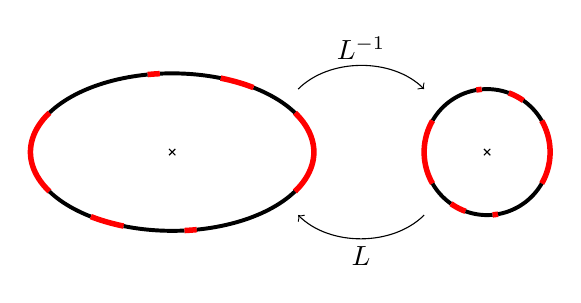
\begin{tikzpicture}[scale=0.4]
\draw (-4-0.1,-0.1) -- (-4+0.1,0.1);
\draw (-4-0.1,0.1) -- (-4+0.1,-0.1);
\draw [line width = 0.7mm,red,domain=-30:30] plot ({-4 + 4.5 * cos(\x)}, {2.5 * sin(\x)});
\draw [line width = 0.5mm,black,domain=30:55] plot ({-4 + 4.5 * cos(\x)}, {2.5 * sin(\x)});
\draw [line width = 0.7mm,red,domain=55:70] plot ({-4 + 4.5 * cos(\x)}, {2.5 * sin(\x)});
\draw [line width = 0.5mm,black,domain=70:95] plot ({-4 + 4.5 * cos(\x)}, {2.5 * sin(\x)});
\draw [line width = 0.7mm,red,domain=95:100] plot ({-4 + 4.5 * cos(\x)}, {2.5 * sin(\x)});
\draw [line width = 0.5mm,black,domain=100:150] plot ({-4 + 4.5 * cos(\x)}, {2.5 * sin(\x)});
\draw [line width = 0.7mm,red,domain=150:210] plot ({-4 + 4.5 * cos(\x)}, {2.5 * sin(\x)});
\draw [line width = 0.5mm,black,domain=210:235] plot ({-4 + 4.5 * cos(\x)}, {2.5 * sin(\x)});
\draw [line width = 0.7mm,red,domain=235:250] plot ({-4 + 4.5 * cos(\x)}, {2.5 * sin(\x)});
\draw [line width = 0.5mm,black,domain=250:275] plot ({-4 + 4.5 * cos(\x)}, {2.5 * sin(\x)});
\draw [line width = 0.7mm,red,domain=275:280] plot ({-4 + 4.5 * cos(\x)}, {2.5 * sin(\x)});
\draw [line width = 0.5mm,black,domain=280:330] plot ({-4 + 4.5 * cos(\x)}, {2.5 * sin(\x)});

\draw (5.9,-0.1) -- (6.1,0.1);
\draw (5.9,0.1) -- (6.1,-0.1);
\draw [line width = 0.7mm,red,domain=-30:30] plot ({6 + 2 * cos(\x)}, {2 * sin(\x)});
\draw [line width = 0.5mm,black,domain=30:55] plot ({6 + 2 * cos(\x)}, {2 * sin(\x)});
\draw [line width = 0.7mm,red,domain=55:70] plot ({6 + 2 * cos(\x)}, {2 * sin(\x)});
\draw [line width = 0.5mm,black,domain=70:95] plot ({6 + 2 * cos(\x)}, {2 * sin(\x)});
\draw [line width = 0.7mm,red,domain=95:100] plot ({6 + 2 * cos(\x)}, {2 * sin(\x)});
\draw [line width = 0.5mm,black,domain=100:150] plot ({6 + 2 * cos(\x)}, {2 * sin(\x)});
\draw [line width = 0.7mm,red,domain=150:210] plot ({6 + 2 * cos(\x)}, {2 * sin(\x)});
\draw [line width = 0.5mm,black,domain=210:235] plot ({6 + 2 * cos(\x)}, {2 * sin(\x)});
\draw [line width = 0.7mm,red,domain=235:250] plot ({6 + 2 * cos(\x)}, {2 * sin(\x)});
\draw [line width = 0.5mm,black,domain=250:275] plot ({6 + 2 * cos(\x)}, {2 * sin(\x)});
\draw [line width = 0.7mm,red,domain=275:280] plot ({6 + 2 * cos(\x)}, {2 * sin(\x)});
\draw [line width = 0.5mm,black,domain=280:330] plot ({6 + 2 * cos(\x)}, {2 * sin(\x)});
\draw[->] (0,2) .. controls (1,3) and (3,3) .. (4,2);
\draw[->] (4,-2) .. controls (3,-3) and (1,-3) .. (0,-2); 
\draw (2,3.3) node {$L^{-1}$};
\draw (2,-3.3) node {$L$};
\end{tikzpicture}
\end{center}
\caption{Change of coordinates to bring our problem back to the case of the unit sphere.}
\end{figure}

%Thus, we consider now the sphere $\sphere$ with a given a subset $X_{\varepsilon} \in \sphere$ that might violate our contractivity constraint. We consider the following property of linear switched systems.

We now know how to compute an upper bound on the JSR when the ``almost invariant" ellipsoid is $\sphere$. Thanks to Property \ref{rem:scaling}, if this is not the case, we can simply perform a change of coordinates mapping this ellipsoid to $\sphere$ and compute the JSR in the new coordinates system instead. To do this, in the next theorem, we bound the measure of violating constraints on $\sphere$ after the change of coordinates, in terms of the measure of the violated constraints on $\sphere \times M^l$ in the original coordinates.

\begin{thm}\label{thm:mainTheorem01}
Let $\gamma^* \in \mathbb{R}_{> 0}$. Consider a set of matrices $\mathcal{M}$, and a matrix $P \succ 0$ satisfying \eqref{eqn:P0}:
\begin{equation}\label{eq:assumptionThm01}
\begin{aligned}
& (A_{j_l} A_{j_{l-1}} \dots A_{j_1} x)^T P(A_{j_l} A_{j_{l-1}} \dots A_{j_1} x) \leq (\gamma^*)^{2l} x^T P x,\\
& \forall\, x \in \sphere \setminus \sphere', \forall\ (j_1, \dotsc, j_l) \in M^l,
\end{aligned}
\end{equation}
for some $\sphere' \subset \sphere$ where $\sigma^{n-1}(\sphere') \leq \varepsilon m^l$. Then, we have 
%%%%%%%Then this contractivity constraint is satisfied on the entire $\sphere$, for a modified contractivity constant $\frac{(\gamma^*)^{2l}}{\alpha(\varepsilon \kappa(P) m^l)}$:
%%%%%%\begin{equation*}\label{eqn:thm01-2}
%%%%%(A_{j_l} A_{j_{l-1}} \dots A_{j_1} x)^T P (A_{j_l} A_{j_{l-1}} \dots A_{j_1} x) \leq \frac{(\gamma^*)^{2l}}{\alpha(\varepsilon \kappa(P) m^l)} x^T P x,\,\, \forall\, x \in \sphere, \, \forall\, (j_1,\dots,j_l) \in M^l,
%%%%%\end{equation*}
$$\rho(\mathcal{M}) \leq \frac{\gamma^{*}}{\sqrt[l]{\alpha \left( \frac{\varepsilon m^l \kappa(P)}{2} \right)}}$$
where $\alpha(\frac{\varepsilon m^l \kappa(P)}{2})$ is given in \eqref{eqn:alphaEpsilon}, and $$\kappa(P) = \sqrt{\frac{\lambda_{\max}(P)^n}{\det(P)}}.$$
\end{thm}

\begin{pf}

The assumption \eqref{eq:assumptionThm01} is a contraction assumption on points of the ellipsoid $E_P$. So far, we have represented points of $E_P$ by their corresponding points on $\sphere$. 

\begin{figure}[H]
\begin{center}
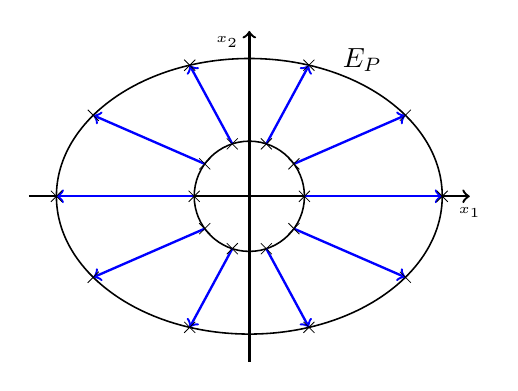
\begin{tikzpicture}[scale=0.7]
\draw[line width=0.2mm,black] (0,0) ellipse [x radius = 3.5cm, y radius =2.5cm];
\draw[line width=0.2mm,black] (0,0) circle [radius=1cm];
\draw[line width=0.3mm,black,->] (-4,0) -- (4,0);
\draw[line width=0.3mm,black,->] (0,-3) -- (0,3);
\draw[black] (4,-0.3) node {\tiny{$x_1$}};
\draw[black] (-0.4,2.8) node {\tiny{$x_2$}};
\draw[black] ({3.5*cos(60)+0.3},{2.5*sin(60)+0.3}) node {$E_P$};
\draw[black] ({cos(60)+0.3},{sin(60)+0.3}) node {$\sphere$};
\foreach \i in {0,...,9}
{
\draw[line width=0.3mm,blue,->] ({cos(\i*36)},{sin(\i*36)}) -- ({3.5*cos(\i*36)},{2.5*sin(\i*36)});
\draw[line width=0.1mm,black] ({cos(\i*36)-0.1},{sin(\i*36)-0.1}) -- ({cos(\i*36)+0.1},{sin(\i*36)+0.1});
\draw[line width=0.1mm,black] ({cos(\i*36)+0.1},{sin(\i*36)-0.1}) -- ({cos(\i*36)-0.1},{sin(\i*36)+0.1});
\draw[line width=0.1mm,black] ({3.5*cos(\i*36)-0.1},{2.5*sin(\i*36)-0.1}) -- ({3.5*cos(\i*36)+0.1},{2.5*sin(\i*36)+0.1});
\draw[line width=0.1mm,black] ({3.5*cos(\i*36)+0.1},{2.5*sin(\i*36)-0.1}) -- ({3.5*cos(\i*36)-0.1},{2.5*sin(\i*36)+0.1});
}
\end{tikzpicture}
\end{center}
\end{figure}


We have $y \in E_P \leftrightarrow x \in \sphere$ with $y = L(x)$, the euclidean norm $y^T y$ becoming $x^T P x$. Hence, \eqref{eq:assumptionThm01} can be rewritten as:
\begin{equation*}\label{eq:assumption2}
\begin{aligned}
& (A_{j_l} A_{j_{l-1}} \dots A_{j_1} x)^T (A_{j_l} A_{j_{l-1}} \dots A_{j_1} x) \leq (\gamma^*)^{2l} x^T x,\\
& \qquad \qquad \qquad \qquad \forall\, x \in E_P \setminus L(\sphere'), \forall\ (j_1, \dotsc, j_l) \in M^l.
\end{aligned}
\end{equation*}

Since we have seen in the previous section a technique to solve the spherical case, we perform now the change of coordinates defined as in \eqref{cholesky} by $L \in \mathcal{L}(\mathbb{R}^n)$ which maps the ellipsoid $E_P$ to the sphere $\sphere$. By defining $\bar{A}_{j_i}=  L^{-1} A_{j_i} L$, assumption \eqref{eq:assumption2} becomes:
\begin{equation*}\label{eq:assumption3}
\begin{aligned}
& (\bar{A}_{j_l} \bar{A}_{j_{l-1}} \dots \bar{A_{j_1}} x)^T P (\bar{A}_{j_l} \bar{A}_{j_{l-1}} \dots \bar{A}_{j_1} x) \leq ({\gamma^*})^{2l} x^T P x, \\
& \forall\, x \in  L^{-1}(E_P \setminus L(\sphere')), \forall\, (j_1,\dots,j_l) \in M^l.
\end{aligned}
\end{equation*}
with $$L^{-1}(E_P \setminus L(\sphere')) = \sphere \setminus \sphere'.$$

In \eqref{eq:assumption3}, we have brought our original contractivity constraints from points of $E_P$ to points of $\sphere$. Now, we recall that the points of the ellipsoid $E_P$ in the initial statement were represented through points of $\sphere$. This sphere becomes after change of coordinates $L$ an ellipsoid $E_{P'}$. Hence, the points of the newly considered level set, $\sphere$, are now represented through points of $E_{P'}$, and \eqref{eq:assumption3} can be rewritten as:
\begin{equation*}\label{eq:assumption4}
\begin{aligned}
& (\bar{A}_{j_l} \bar{A}_{j_{l-1}} \dots \bar{A_{j_1}} x)^T  (\bar{A}_{j_l} \bar{A}_{j_{l-1}} \dots \bar{A}_{j_1} x) \leq ({\gamma^*})^{2l} x^T  x, \\
&  \forall\, x \in  L^{-1}(\sphere \setminus \sphere'), \, \forall\, (j_1,\dots,j_l) \in M^l,
\end{aligned}
\end{equation*}
with $$L^{-1}(\sphere \setminus \sphere') = E_{P'} \setminus L^{-1}(\sphere').$$
\begin{figure}[H]
\begin{center}
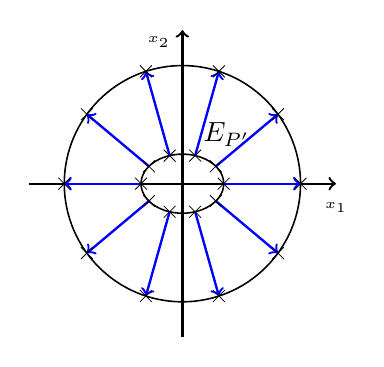
\begin{tikzpicture}[scale=1.5]
\draw[line width=0.2mm,black] (0,0) ellipse [x radius = 0.35cm, y radius =0.25cm];
\draw[line width=0.2mm,black] (0,0) circle [radius=1cm];
\draw[line width=0.3mm,black,->] (-1.3,0) -- (1.3,0);
\draw[line width=0.3mm,black,->] (0,-1.3) -- (0,1.3);
\draw[black] (1.3,-0.2) node {\tiny{$x_1$}};
\draw[black] (-0.2,1.2) node {\tiny{$x_2$}};
\draw[black] ({0.35*cos(60)+0.2},{0.25*sin(60)+0.2}) node {$E_{P'}$};
\draw[black] ({cos(60)+0.2},{sin(60)+0.2}) node {$\sphere$};
\foreach \i in {0,...,9}
{
\draw[line width=0.3mm,blue,->] ({0.35*cos(\i*36)},{0.25*sin(\i*36)}) -- ({cos(\i*36)},{sin(\i*36)});
\draw[line width=0.1mm,black] ({cos(\i*36)-0.05},{sin(\i*36)-0.05}) -- ({cos(\i*36)+0.05},{sin(\i*36)+0.05});
\draw[line width=0.1mm,black] ({cos(\i*36)+0.05},{sin(\i*36)-0.05}) -- ({cos(\i*36)-0.05},{sin(\i*36)+0.05});
\draw[line width=0.1mm,black] ({0.35*cos(\i*36)-0.05},{0.25*sin(\i*36)-0.05}) -- ({0.35*cos(\i*36)+0.05},{0.25*sin(\i*36)+0.05});
\draw[line width=0.1mm,black] ({0.35*cos(\i*36)+0.05},{0.25*sin(\i*36)-0.05}) -- ({0.35*cos(\i*36)-0.05},{0.25*sin(\i*36)+0.05});
}
\end{tikzpicture}
\end{center}
\end{figure}
To reason on the (spherical) measure of violating set in the new coordinates, we project $E_{P'}$ on the unit sphere; $L^{-1}(\sphere')$ becomes $\proj_\sphere(L^{-1}(\sphere'))$.

We now show how to relate $\sigma^{n-1}(\proj_\sphere(L^{-1}(\sphere')))$ to $\sigma^{n-1}(\sphere')$, measure of the violating set in the initial coordinates. Consider $\sphere^{\sphere'}$, the sector of $\ball$ defined by $\sphere'$. We denote $C:= L^{-1}(\sphere')$ and $C':=\proj_\sphere(L^{-1}(\sphere'))$. We have $\proj_{\sphere}(C) = C'$ and $\sphere^{C'} \subset \mathcal{H}_{1/ \lambda_{\min}(L^{-1})}(C),$
where $\mathcal{H}_{1/ \lambda_{\min}(L^{-1})}$ is the homothety of ratio $1/ \lambda_{\min}(L^{-1})$. This leads to:
$$\sigma^{n-1}(C') = \lambda \left( \sphere^{C'} \right) \leq \lambda \left( \mathcal{H}_{1/ \lambda_{\min}(L^{-1})}(E_{P'}^{C}) \right).$$ Then, the following holds: \begin{eqnarray}
\nonumber\sigma^{n-1}(C') &\leq& \frac{1}{\lambda_{\min}(L^{-1})^n}\lambda(E_{P'}^{C}) \\
\nonumber &\leq&\frac{1}{\lambda_{\min}(L^{-1})^n} \lambda \left( L^{-1}(\sphere^{\sphere'}) \right)\\ 
\label{eqn:lt} &=&\frac{|\det(L^{-1})|}{\lambda_{\min}(L^{-1})^n}\lambda \left( \sphere^{\sphere'} \right),\\
\label{eqn:map1} &=&\sqrt{\frac{\lambda_{\max}(P)^n}{\det(P)}}\sigma^{n-1}(\sphere')
\end{eqnarray}
where \eqref{eqn:lt} follows from the fact that
$$ \lambda(Q(X)) = |\det(Q)| \lambda(X),$$
for any set $X \subset \mathbb{R}^n$ and $Q \in \mathcal{L}(\mathbb{R}^n)$ (see e.g. \cite{rudin}).

Finally, thanks to the Property~\ref{rem:scaling}, we even have:
\begin{equation}\label{eqn:P1}
\begin{aligned}
& (A_{j_l} A_{j_{l-1}} \dots A_{j_1} x)^T P (A_{j_l} A_{j_{l-1}} \dots A_{j_1} x) \leq (\gamma^*)^{2l} x^T P x, \\ 
& \forall\, x \in \sphere \proj_\sphere(L(\sphere')), \,\forall\, (j_1,\dots,j_l) \in M^l.
\end{aligned}
\end{equation}
with $$\sigma^{n-1} \left(  \proj_\sphere(L(\sphere')) \right) \leq \sqrt{\frac{\lambda_{\max}(P)^n}{\det(P)}}\sigma^{n-1}(\sphere'), $$ which gives us our theorem.
%%Then, if we let $E':=L^{-1} V_\sphere$, where $L$ is the linear transformation mapping $E_P$ to $\sphere$, we get: $$\sigma_P(E') = \sigma^{n-1}(V_\sphere), and the result of the theorem follows.
\end{pf}

\end{subsection}